% !TEX root = ./main.tex

\section{Introduction}
% \subsection{Motivation}

group theoretical methods in machine learning by Kondor \cite{kondorGroupTheoreticalMethods2008}.
diffusion kernel on graphs \cite{kondorDiffusionKernelsGraphs2002}

Many insightful and powerful models, like adiabatic quantum computation \cite{farhiQuantumComputationAdiabatic2000}, quantum random walks \cite{childsQuantumInformationProcessing2004} 
% \cite{ambainisOnedimensionalQuantumWalks2001}, 

\subsection{Preliminary and Notations}
a datum $\vbx:= (x_1,x_2,\dots,x_d) \in \realnumber^d$ is a vector where $d$ is the number of \emph{features};
dataset $\qty{(\vbx^{(i)}, y^{(i)})}^{m}_{i=1}$ where the \emph{label} $y\in\Sigma$ with some (discrete set) alphabet/category $\Sigma$. 
for binary classification, we have $\Sigma=\qty{-1,1}$,
$\Omega$;
computational basis $\ket{z}$ with $z\in \qty{1,2,\dots,2^n}$ where $n$ is the number of qubits,
the binary representation $\ket{\vbx}=\ket{x_1,x_2,\dots,x_n},x_j\in \qty{0,1}$.
$\ket{0}^n$, $\ket{\pm}$.
graph $\graph$, group $\group$
% \subsubsection{Support Vector Machine (SVM)}
% \subsubsection{Kernel trick}
% \subsubsection*{Hilbert space}
\begin{definition}[Inner product]\label{def:inner_product}
	\emph{inner product} $\expval{\vbx,\vbx'}$.
	Dirac notation $\braket{\vbx}{\vbx'}$
\end{definition}
`similarity' between two vectors ?
\begin{definition}[Hilbert space]\label{def:hilbert_space}
	\emph{Hilbert space} $\hilbertspace$ induced by \emph{inner product}
\end{definition}

\subsection{Terminology: SVM and Kernel trick}\label{sec:svm}
\emph{supervised learning} 
\footnote{unsupervised learning}
\subsubsection*{Support Vector Machine (SVM)}
training stage, classification stage.
exponentially large space;
\emph{hyperplane} $(\vb{w},b)$ parametrized by a normal vector $\vb{w}\in\realnumber^n$ and a \emph{bias} term $b\in\realnumber$. in the (high-dimensional) \emph{feature space}.
maximize the \emph{margin} [ref]
\begin{equation}
	f^* = \arg \max_f  L(y,\tilde{y}) + \norm{}
\end{equation}
where the loss function $L$, slackness. called \emph{support vector}.

\subsubsection*{Kernel trick (method)}
\emph{kernel trick}: \emph{feature map} the input data to higher dimension such that the data are linearly separatable in this feature space.
only depend on the inner product to avoid the expensive (exponential) calculation. [ref]
\begin{definition}[Kernel function]\label{def:kernel}
	a \emph{kernel function} (mapping) $\kernel: \Omega\times\Omega\to\realnumber$,
	is defined as \nameref{def:inner_product}
	% a \emph{(feature) mapping} $\phi:\Omega\mapsto\hilbertspace_\kernel$
	\begin{equation}
		\kernel(\vbx,\vbx') = \langle \Phi(\vbx),\Phi(\vbx') \rangle_{\hilbertspace}
		\label{eq:kernel_classical}
	\end{equation}
	w.r.t a \nameref{def:feature_map_classical} $\Phi(\vbx)$.
\end{definition}
\begin{remark}
	A function $\kernel$ ($k$) is a valid kernel (in machine learning) if and only if? the matrix $\kernel(x,x')$ is symmetric and \emph{positive semi-definite} (PSD, p.s.d).
\end{remark}
\begin{definition}[Feature map]\label{def:feature_map_classical}
	The \emph{feature map} is a function (mapping)
	\begin{equation}
		\Phi(\vbx) : \Omega \to \hilbertspace_{\kernel}
		\label{eq:feature_map_classical}
	\end{equation}
	from a low dimensional space non-linearly in to a high dimensional \nameref{def:hilbert_space} $\hilbertspace$ which is commonly referred to as the \emph{feature space}.
	For example, $\Phi(\vbx):\realnumber^d \to \realnumber^n$ with $n\gg d$.
\end{definition}
\begin{figure}[!ht]
	\centering
	\begin{subfigure}{0.3\textwidth}
	\centering
		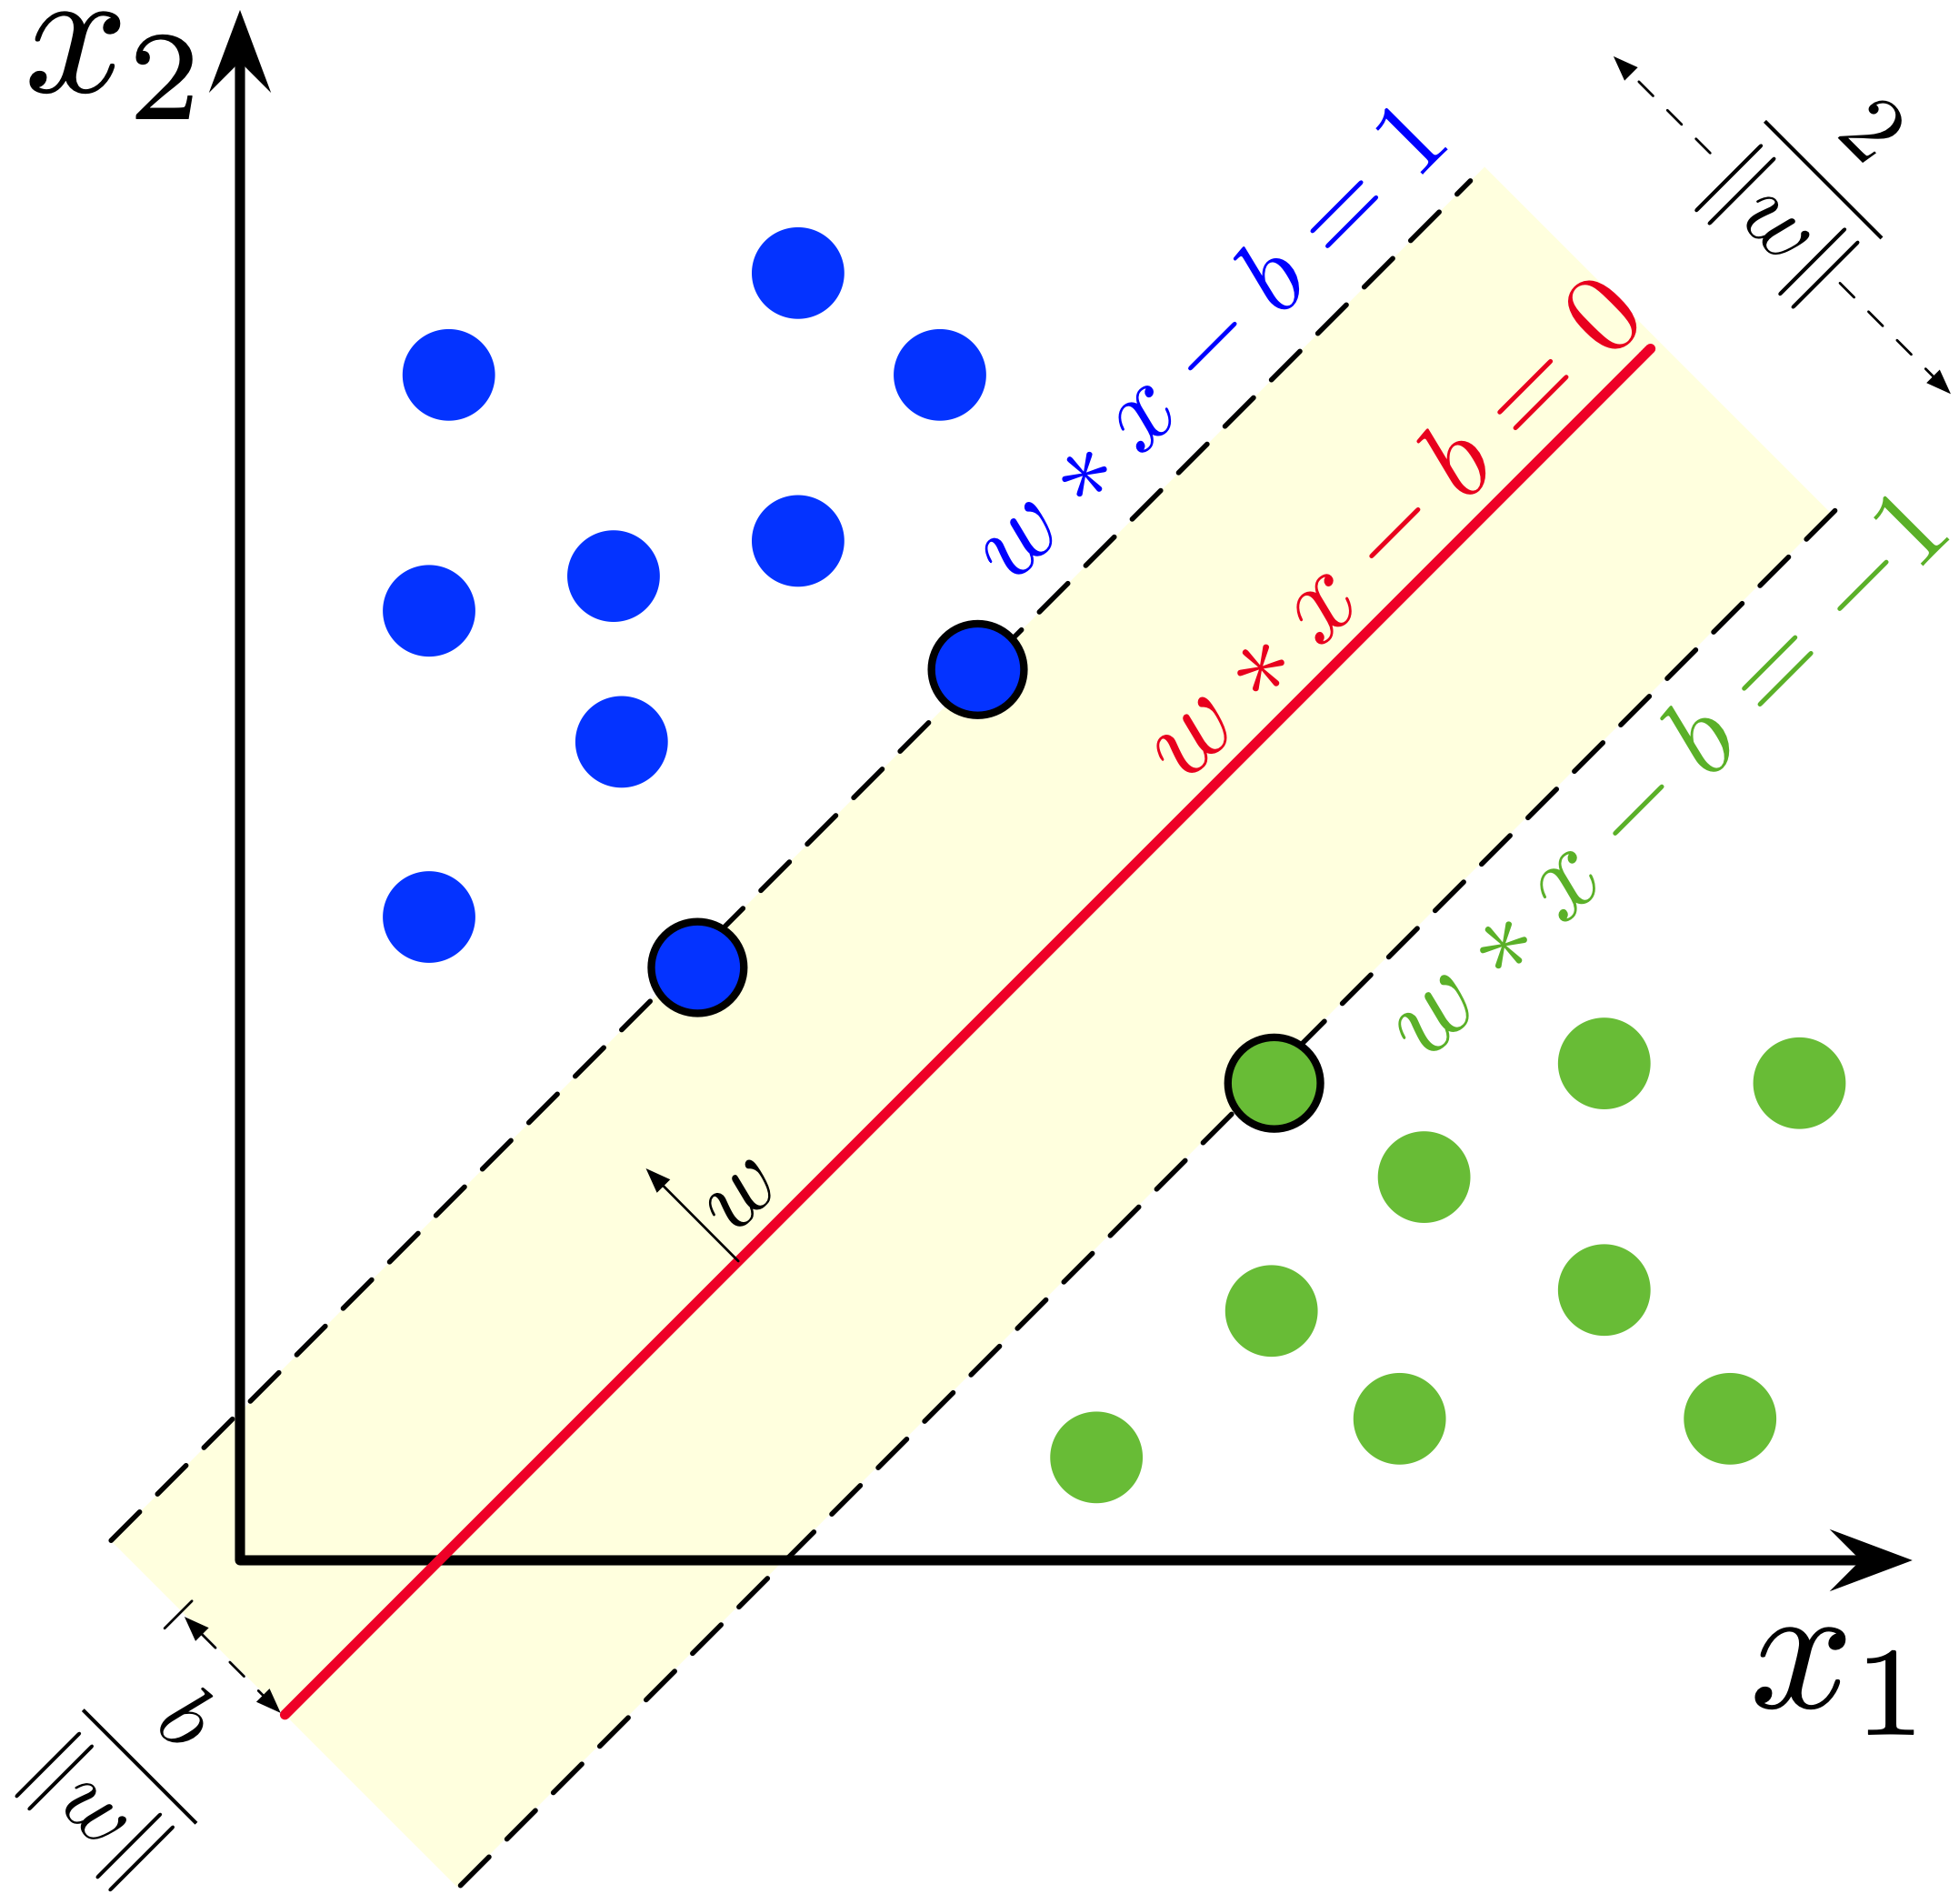
\includegraphics[width=.9\linewidth]{SVM_margin.png}
		\caption{linearly separable SVM}
	\end{subfigure}
	\begin{subfigure}{0.68\textwidth}
	\centering
		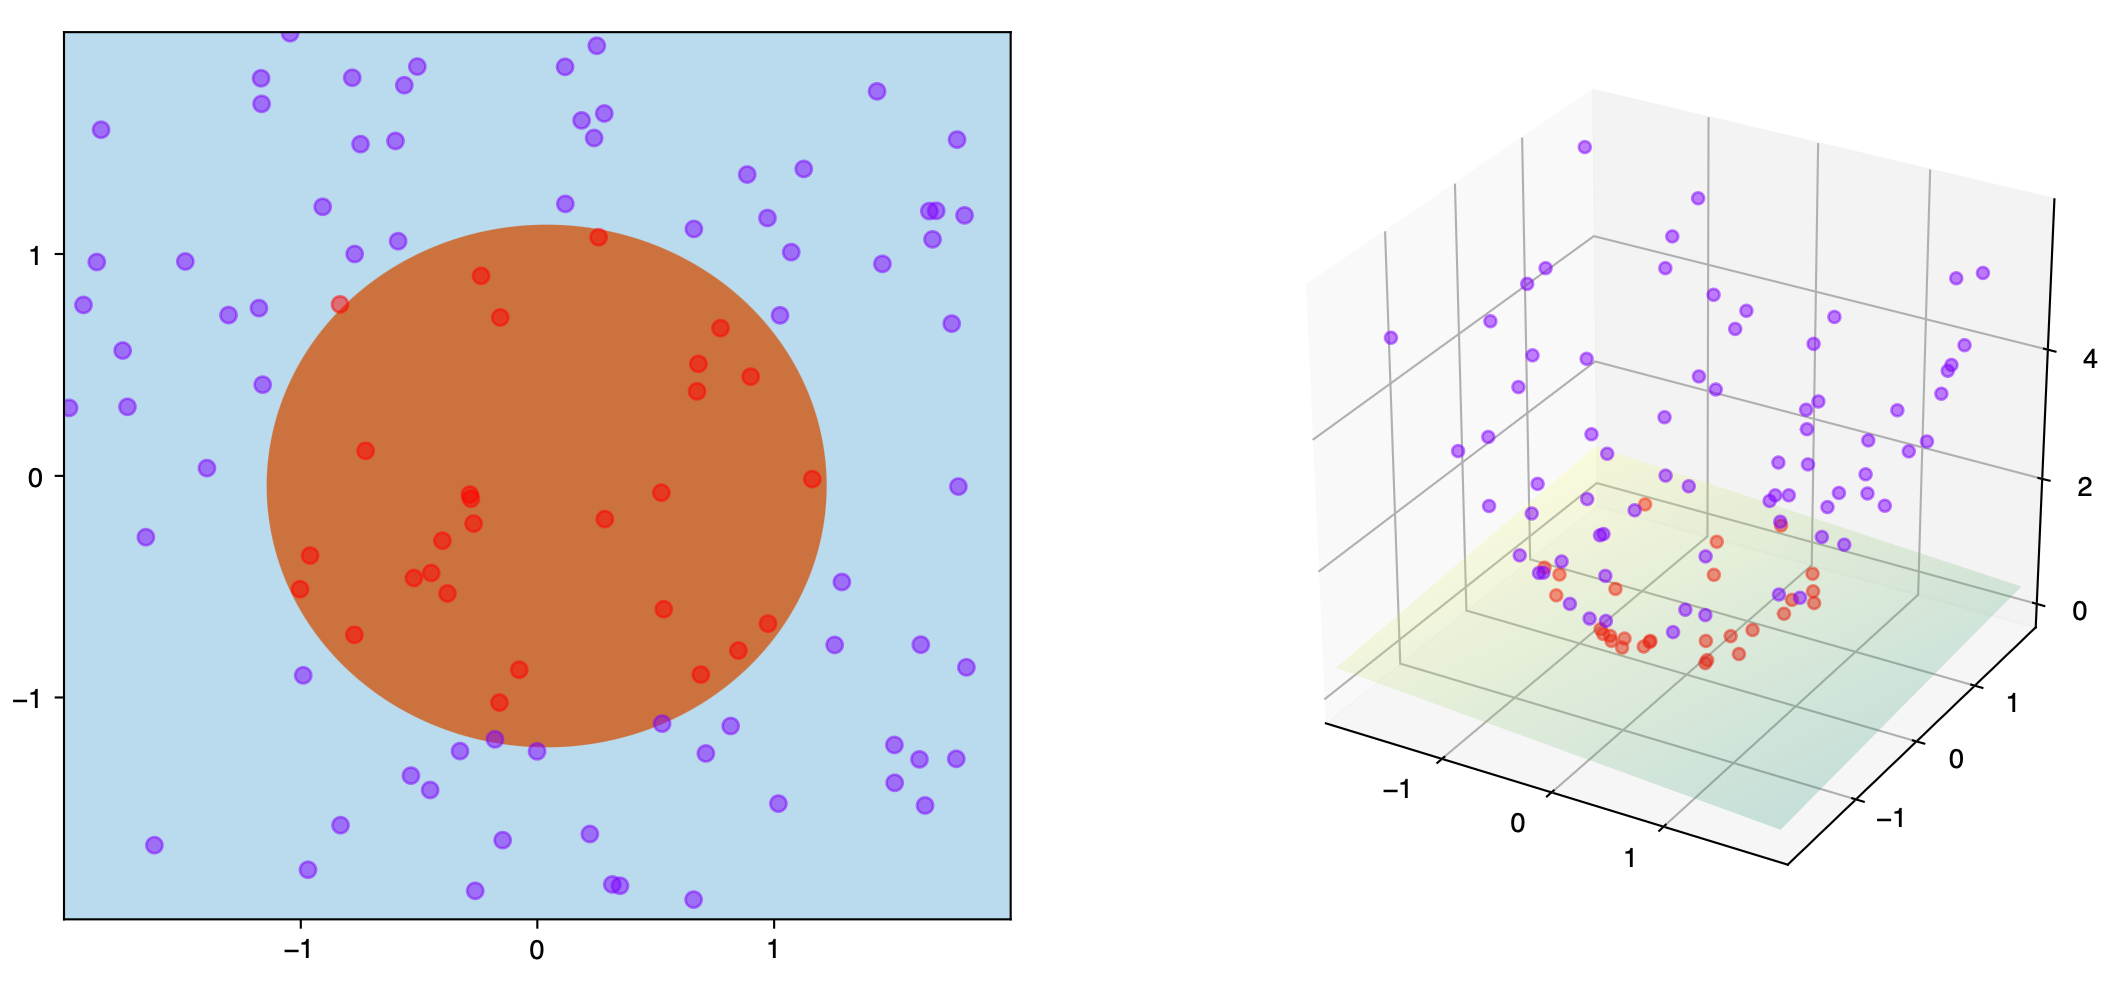
\includegraphics[width=.9\linewidth]{kernel_trick_idea.png}
		\caption{kernel trick idea: SVM with kernel given by $\phi(\vbx:=(a, b)) = (a, b, a^2 + b^2)$ and thus $\kernel(\vbx,\vb{y})=\vbx\cdot \vb{y}+\norm{x}^2 \norm{y}^2$ that only depends on inner product. The training points are mapped to a 3-dimensional space where a separating hyperplane can be easily found. (from Wikipedia: Kernel method)}	
	\end{subfigure}
\end{figure}
% \begin{figure}[!ht]
% 	\centering
% 	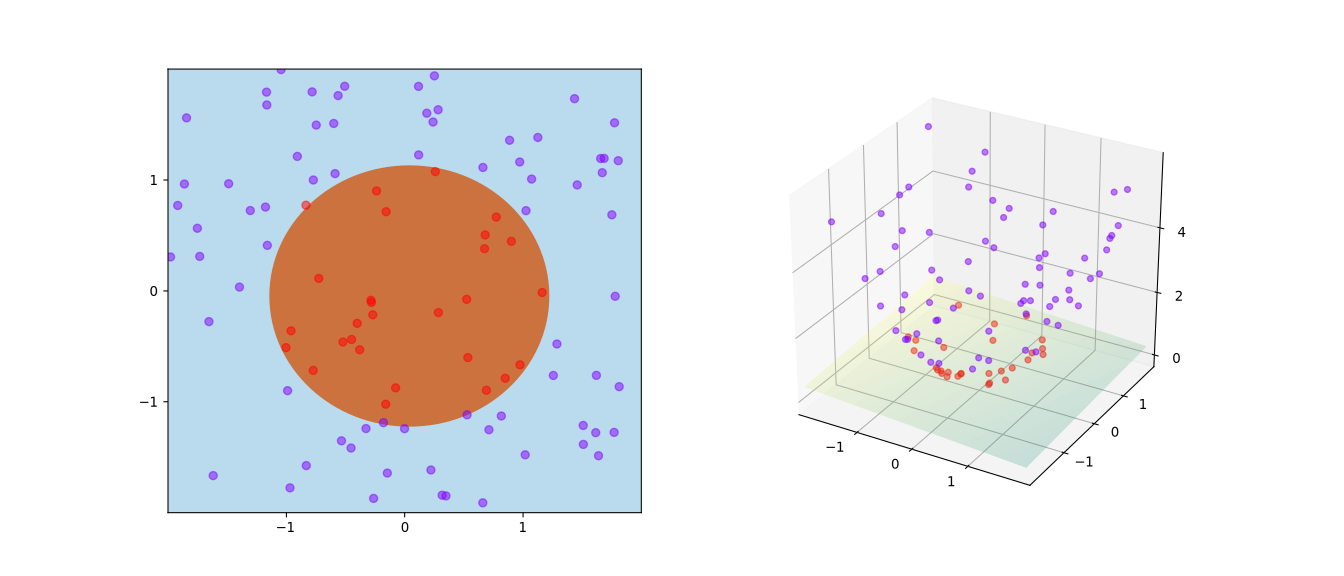
\includegraphics[width=0.8\linewidth]{Kernel_trick_idea.png}
% 	\caption{kernel trick idea: SVM with kernel given by $\phi(\vbx:=(a, b)) = (a, b, a^2 + b^2)$ and thus $\kernel(\vbx,\vb{y})=\vbx\cdot \vb{y}+\norm{x}^2 \norm{y}^2$ that only depends on inner product. The training points are mapped to a 3-dimensional space where a separating hyperplane can be easily found. (from Wikipedia: Kernel method)}
% \end{figure}
Some common kernels: 
\begin{itemize}
	\item polynomial kernel:
	\item radial:
	\item \emph{Gaussian (radial basis) kernel}:
	\begin{equation}
		\kernel(\vbx,\vbx') = 
		\exp(-\frac{\norm{\vbx-\vbx'}}{2\sigma^2})
	\end{equation}
\end{itemize}

\begin{definition}[Reproducing Kernel Hilbert Space]
	It is well known that any continuous, symmetric, positive definite \nameref{def:kernel} has corresponding Hilbert space $\hilbertspace$, called the \emph{Reproducing Kernel Hilbert Space} (RKHS),
	which induces a \nameref{def:feature_map_classical}
	satisfying \cref{eq:kernel_classical}.
\end{definition}
\begin{theorem}[Representer theorem]
	?
\end{theorem}

\section{Graph Kernels and Quantum Random Walks}
Largely, this development was driven by the empirical success of supervised learning of vector-valued data or image data. However, in many domains, such as chemo- and bioinformatics, social network analysis or computer vision, observations describe relations between objects or individuals and cannot be interpreted as vectors or fixed grids; instead, they are naturally represented by graphs.
\cite{kriegeSurveyGraphKernels2020}
graph-structured data is to make use of graph kernels—functions which measure the similarity between graphs.
\textbf{How similar are two graphs?}
\textbf{How similar are two nodes of a graph?}

\subsection{Diffusion kernel of a graph (between a pair of vertices)}
\cite{kondorDiffusionKernelsGraphs2002}.
generalize to regularization: 
We propose a family of regularization operators (equivalently, kernels) on graphs that include Diffusion Kernels as a special case, and show that this family encompasses all possible regularization operators invariant under permutations of the vertices in a particular sense.
\cite{smolaKernelsRegularizationGraphs2003}
with Euclidean space $\Omega = \realnumber^m$

\begin{definition}[Adjacency matrix]\label{def:adjacency_matrix}
	Given a (undirected, unweighted) graph $\graph(V,E)$, its \emph{adjacency matrix} $\hat{A}$ is defined as
	\begin{equation}
		\hat{A}(v,v') : = 
		\begin{cases}
			1, & (v,v') \in E \\
			0, & \text{otherwise}
		\end{cases}
	\end{equation}
	where the matrix entry is 1 if the two vertices $v,v'$ (labels of the column and the row) are connected by an edge, otherwise the entry is 0.
\end{definition}
\begin{definition}[Graph Laplacian]\label{def:graph_laplacian}
	With the adjacency matrix $\hat{A}$, the graph Laplacian is
	\begin{equation}
		\llaplacian:=\hat{A}-\hat{D}	
		% \Longleftrightarrow
		% \hhat_0=\frac{\phat^2}{2m}
		% % \sim \nabla^2
		% =-\frac{\hbar^2\nabla^2}{2m}
		% % \Longleftrightarrow \dlagrangian ?
	\end{equation}
	where $\hat{D}_{v,v}:=\deg(v)$ is its diagonal degree matrix.
	The adjacency matrix and graph Laplacian of weighted graphs can be defined analogously.
\end{definition}
\begin{remark}
	Graph Laplacian $\llaplacian$ is the 
	discrete version of (continuous) Laplacian operator $\laplacian$.
	\cite{chungSpectralGraphTheory1997}
\end{remark}
\begin{lemma}
	matrix exponential of any ? $\hhat$ i.e., $e^{\beta \hamiltonian}$, is a valid kernel (PSD). [to verify for $e^{-\ii t\hamiltonian}$]
\end{lemma}
\begin{definition}[Diffusion kernel]\label{def:diffusion_kernel}
	The \emph{diffusion kernel} of a graph w.r.t a pair of vertices $(v,v')$
	is $\kernel(v,v'):V(G)\to \realnumber$, i.e.,
	\begin{equation}
		\kernel(v,v') := 
		\qty[\sum_{k}\frac{\beta^k}{k!}\llaplacian^k]_{v,v'}  =
		\qty[e^{\beta \llaplacian}]_{v,v'} 
	\end{equation}
	where $\Omega$ is the set of vertices of graph $G$.
\end{definition}

\subsubsection{Diffusion, heat equation, and random walk}
The continuous-time random walk on $G$ is defined as the \textbf{solution of the differential equation}
\begin{equation}
	\dv{t} p_j(t)
	=
	\sum_{k\in V} \llaplacian_{jk} \ p_k(t),
	\label{eq:continuous_time_random_walk}
\end{equation}
where $p_j(t)$ denotes the probability associated with vertex $j$ at time $t$
and $\llaplacian$ is \nameref{def:graph_laplacian}.
Since the columns of $\llaplacian$ sum to 0,
% \begin{equation}
% 	\dv{t} \sum_{j\in V} p_j (t) = 
% 	\sum_{j,k\in V} \llaplacian_{jk}  p_k(t) = 0
% \end{equation}
% which shows that 
an initially normalized distribution remains normalized:
the evolution of the continuous-time random walk for any time $t$ is a \emph{stochastic process}.
\emph{random walk} (discrete-space, discrete-time), 
\emph{heat equation} 
\begin{equation}
	u_t = \alpha \laplacian u \equiv \alpha \Delta u
	\label{eq:heat_equation}
\end{equation}
continuous-space (continous-time)
the solution to \cref{eq:heat_equation} is called heat kernel $\kernel(t;x,y)=\frac{1}{4\pi t} e^{-\abs{x-y}^2/4t}$ (Gaussian).

\subsection{Continuous-time quantum random walk}\label{sec:ct_quantum_walk}
The continuous-time quantum random walk \cite{childsExampleDifferenceQuantum2002} is the quantum analogue of classical diffusion (continuous-time random walk).
By a direct observation, \cref{eq:continuous_time_random_walk} is very similar to the time-dependent (evolution) schrodinger equation governed by a Hamiltonian operator $\hamiltonian$
\begin{equation}
	i\hbar \dv{t} \ket{\psi} = \hamiltonian \ket{\psi}
	\label{eq:evolution}
\end{equation}
except that the factor of $\ii\hbar$.
\begin{definition}[Quantum propagator]\label{def:quantum_propagator}
	\emph{Quantum propagator}, \emph{transition amplitude}.
	Interestingly, this quantity is also called \emph{quantum kernel} (much earlier than the concept of kernel tricks in machine learning), 
	\begin{equation}
		\mel{I}{e^{-\ii t \hamiltonian}}{F}
		=
		\mel{I}{\U}{F}
	\end{equation}
	The quantum propagator can be evaluated by \emph{path integral (Lagrangian) formalism} (see \cref{sec:lagrangian}).
\end{definition}

\subsection{Graph kernels of a pair of graphs}
random walk kernel
\cite{vishwanathanGraphKernels2010}
quantum kernel
\cite{baiQuantumJensenShannon2015}
survey
\cite{kriegeSurveyGraphKernels2020}
\begin{definition}[Graph kernel]\label{def:graph_kernel}
	Given a pair of graphs $(G,G')$,
	a \emph{graph kernel} is a function (mapping)
	$\kernel(G,G'): \qty{ \graph } \to \realnumber$
\end{definition}
\cite{chungSpectralGraphTheory1997}
\begin{definition}[Product of graphs]\label{def:product_graphs}
	\emph{direct product of graphs};
	\begin{equation}
		G(V,E)\times G'(V',E') 
		: = \qty{(v,v')\in V\times V',((v,v'),(w,w'))\in E \wedge??}
	\end{equation}
	\emph{tensor product of graphs};
	\begin{equation}
		G\otimes G' := \qty{ \vee }
	\end{equation}
	\emph{Cartisan product of graphs};
	\begin{equation}
		G\times G' = \qty{}
	\end{equation}
	\emph{Kronecker product};
	\emph{factor graph};
	\emph{Hadamard product};
\end{definition}
\begin{remark}
	A natural question to ask is the following: Since diffusion can be viewed as a \textbf{continuous time} limit of random walks, can the ideas behind the random walk kernel be extended to diffusion? Unfortunately, the Laplacian of the product graph does not decompose into the Kronecker product of the Laplacian matrices of the constituent graphs; this rules out a straightforward extension.
	discrete-time quantum random walk (need coin space) \cite{ambainisCoinsMakeQuantum2005} \cite{childsQuantumInformationProcessing2004};
	Szegedy's walk formalism.
	\cite{szegedySpectraQuantizedWalks2004}
\end{remark}
\begin{remark}
	for diffusion processes on factor graphs the kernel on the factor graph is given by the product of kernels on the constituents, that is 
	\begin{equation}
		k((i, i'), (j, j')) = k(i, j) k' (i' , j' ).
	\end{equation}
\end{remark}

\subsection{Discrete-time quantum random walk}
\emph{Discrete-time quantum random walk} is the quantum analogy of random walk

\subsection{Relation and examples}
\subsubsection{Line}
(classical) diffusion kernel of a 1-dimensional lattice (line)
\begin{equation}
	\kernel(v,v') = 
\end{equation}
\nameref{def:quantum_propagator} (quantum kernel)
\begin{align}
	\tilde{\kernel}(z_F,z_I) = 
	\mel{z_F}{e^{-\ii t\hhat_0 }}{z_I}
	&=\sum_{p=1}^{N} 
	e^{-\ii t 2\cos(\frac{2\pi}{N}p) +\ii \frac{2\pi}{N} p(z_I-z_F)} 
	\\
	&
	% \approx \frac{1}{2\pi} \int_{\pi}^{\pi} e^{\ii p d -2\ii t cos(p)} \dd{p} 
	\approx e^{2\ii t} (-\ii)^{d} J_{d} (2t)
	\label{eq:ctqrw_kernel}
\end{align}
\begin{figure}[!ht]
	\centering
	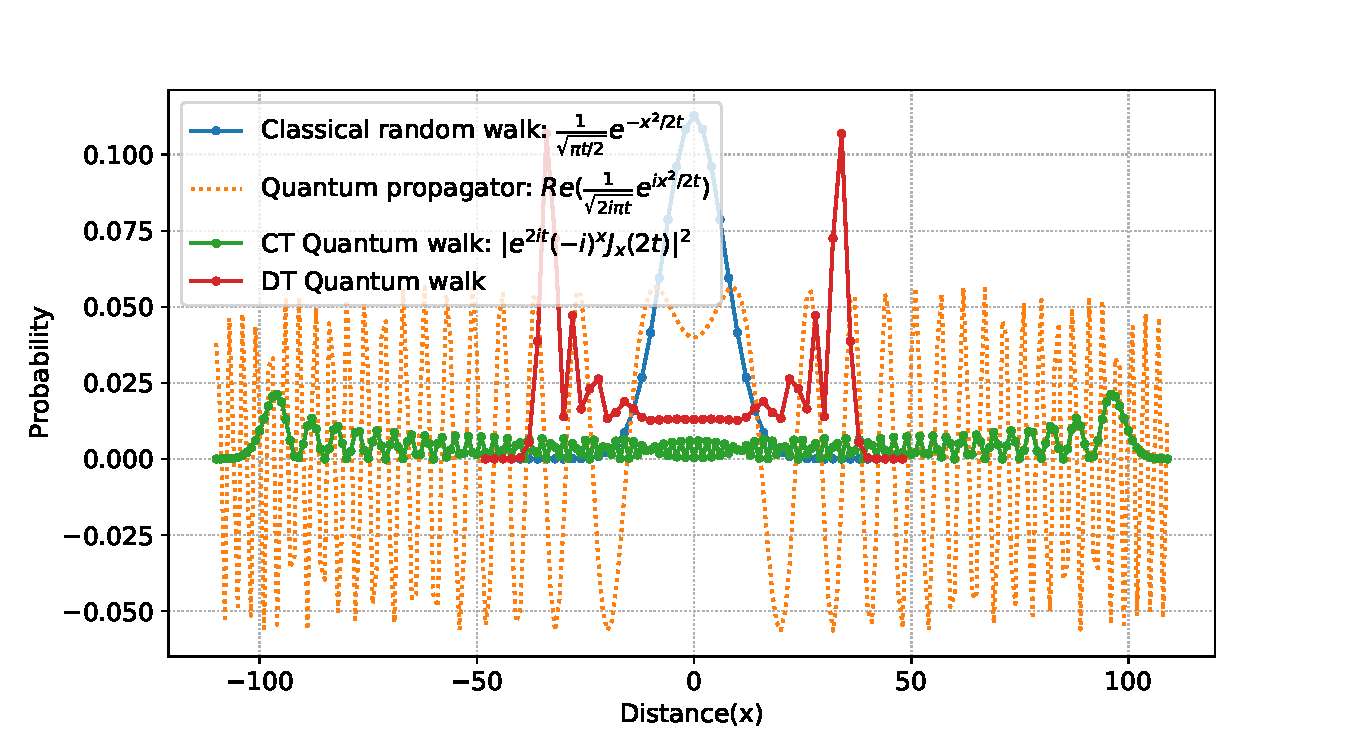
\includegraphics[width=.7\linewidth]{walk_propagator_1d.pdf}
	\caption{}
\end{figure}
\begin{remark}
    The random walk on this graph starting from the origin (in either continuous or discrete time)
    typically moves a distance proportional to $\sqrt{t}$ in time $t$.
	In contrast, the quantum random walk spreads as a wave packet with speed 2.
\end{remark}

\subsubsection{Tree}
\subsubsection{Hyercube}
\subsubsection{Cayley graphs}
\begin{definition}[Cayley graph]\label{def:cayley_graph}
	Cayley graph is a graph that encodes the abstract structure of a group. 
\end{definition}

\section{Quantum Advantages and Speedups}\label{sec:speedup}
A quantum version of this approach has already been proposed in \cite{rebentrostQuantumSupportVector2014},
where an exponential improvement can be achieved if data is provided in a coherent superposition. 
\begin{remark}
	However, when data is provided in the conventional way, i.e. from a classical computer, then the methods of [15] cannot be applied.
\end{remark}
input model, quantum RAM;
quantum-inspired \cite{tangQuantuminspiredClassicalAlgorithm2019}

% \subsection{Quantum Machine Learning: SVM and QKE}
\subsection{Related works}\label{sec:qke}

\subsubsection{Quantum SVM and kernel tricks}
Quantum version of SVM was proposed \cite{rebentrostQuantumSupportVector2014} to exploit the power of quantum computer.
Naturally, the \emph{quantum kernel estimation}
\cite{schuldQuantumMachineLearning2019}
\cite{havlicekSupervisedLearningQuantum2019} 
is studied to enhance the performance of quantum SVM.
\begin{definition}[Quantum feature map]\label{def:quantum_feature_map}
	the quantum state space (Hilbert space) as the feature space to still obtain a quantum advantage
	mapping the input data non-linearly to a quantum state (density matrix) 
	\begin{equation}
		\Phi(\vbx): \Omega \to \dyad{\Phi(\vbx)},
		\label{eq:quantum_feature_map}
	\end{equation}
	the direct quantum analogy of classical \nameref{def:feature_map_classical}.
	On quantum computers, the quantum feature map $\Phi(\vbx)$ is realized by applying a unitary quantum circuit $\U_{\Phi(\vbx)}$ to a reference state $\ket{0^n}$.
\end{definition}

\subsubsection{Explicit method (Quantum Variational Classification)}
variational quantum circuit: generates a separating hyperplane in the quantum feature space
\begin{enumerate}
	\item $\vbx\in\Omega$ (feature) mapped to a quantum state by applying a unitary circuit $U_{\Phi(\vbx)}$ to a reference (initial) state $\ket{0}^n$
	\item a short depth quantum circuit $W(\vb{\theta})$
	\item for binary classification, apply a binary measurement $\qty{M_y}=2^{-1}(\identity + y \vb{f})$?
	\item to obtain the empirical distribution $p_y(\vbx)$, perform repeated measurement shots.
	then assign the label according to $p_y$?
\end{enumerate}

\subsubsection{Implicit method (Quantum Kernel Estimation)}
estimate the kernel function quantumly and implement a conventional SVM.
Rather than using a variational quantum circuit to generate the separating hyperplane, we use a classical SVM for classification.
\begin{enumerate}
	\item the kernel $\kernel(\vbx,\vbx')$ is estimated on a quantum computer
	\item the quantum computer is used a second time to estimate the kernel for a new datum (test) $\vb{s}\in S$ with all the support vectors.
\end{enumerate}

\textbf{The kernel entries are the fidelities between different feature vectors.}
The overlap can be estimated directly from the transition amplitude 
\begin{definition}[Quantum kernel estimation]\label{def:quantum_kernel}
	The \emph{quantum kernel estimation} is the \emph{Hilbert-Schmidt} \nameref{def:inner_product} between density matrices
	\begin{equation}
		\kernel(\vbx,\vbx') 
		= \Tr\qty(\dyad{\Phi(\vbx)}\cdot \dyad{\Phi(\vbx')})
		= \abs{\braket{\Phi(\vbx)}{\Phi(\vbx')}}^2 = 
		\abs{\matrixel{0^n}{\U^\dagger_{\Phi(\vbx)} \U_{\Phi(\vbx')}}{0^n}}^2.
	\end{equation}
	exactly the \nameref{def:quantum_propagator}.
\end{definition}
measure the final state in the Z-basis R-times and record the number of $\ket{0^n}$.
The frequency of this string is the estimate of the transition probability.
The kernel entry is obtained to an additive sampling error of $\tilde{\epsilon}$ when $\bigO(\tilde{\epsilon}^{-2})$ shots are used.

\begin{theorem}[\cite{childsExponentialAlgorithmicSpeedup2003}]
	There exists exponential (classiacl-quantum) separation with respect to query complexity under the adjacency matrix (graph) model. (glued tree)
\end{theorem}
\cite{zhengSpeedingLearningQuantum2022};
robust, provable speedup
\cite{liuRigorousRobustQuantum2021}

\subsubsection{Quantum graph kernel}
quantum graph kernel defined in terms of Jensen Shannon
\cite{baiQuantumJensenShannon2015}

\subsubsection{Quantum diffusion map}
Inspired by random walk on graphs, \emph{diffusion map} (DM) is a class of \textbf{unsupervised} machine learning that offers automatic identification of \textbf{low-dimensional data structure hidden in a high dimensional dataset} \cite{sornsaengQuantumDiffusionMap2021}.
Though both are machine learning techniques, diffusion map (for dimension reduction) is the `reverse direction' of the kernel method.


\subsection{Provable: Symmetries, graph properties}
structure is required for quantum speedup
\cite{aaronsonNeedStructureQuantum2014}
symmetric functions rule out exponential speedup
\cite{ben-davidSymmetriesGraphProperties2020}

\subsubsection{Permutation, symmetry, and speedup}
\begin{figure}[!ht]
	\centering
	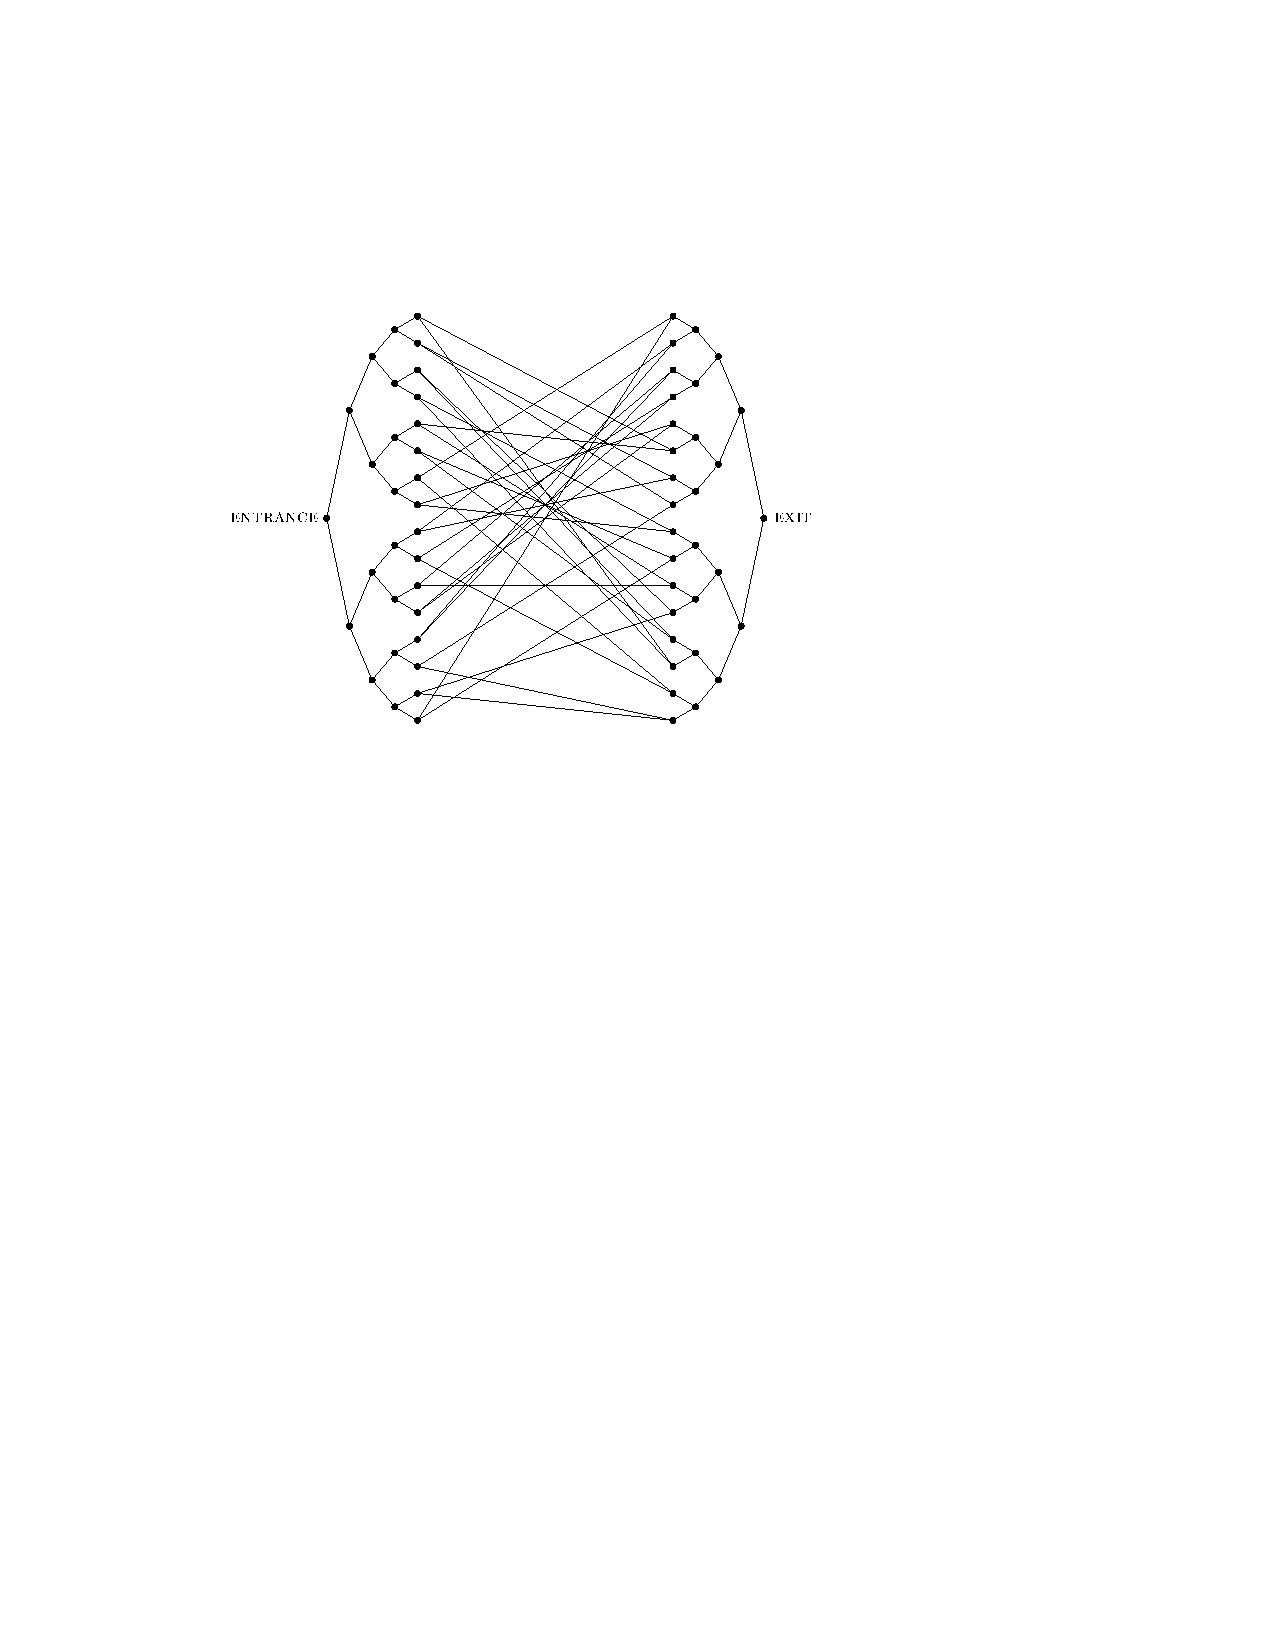
\includegraphics[width=.6\linewidth]{glued_tree.pdf}
	\caption{\cite{childsExponentialAlgorithmicSpeedup2003}}
\end{figure}

\subsubsection{FFT and QFT}
\cite{kondorGraphletSpectrum2009};
quantum linear algebra (qMAT) [ref]: HHL, matrices multiplication, matrix inversion, matrix exponentiation, FFT by quantum algorithms
\cite{sornsaengQuantumDiffusionMap2021}

\subsection{Heuristic: Groups, invariance, symmetries of physical systems}
hidden subgroup problem solved by quantum Fourier transformation\cite{childsQuantumAlgorithmsAlgebraic2010};
rigorous and robust quantum speedup with Discret Logarithm (DLOG) problem \cite{liuRigorousRobustQuantum2021}

\subsubsection{Groups, symmetries in physics}
covariant 
\cite{glickCovariantQuantumKernels2021}
group theory, 
\cite{kondorGroupTheoreticalMethods2008};
symmetries in physics
\cite{bogatskiyLorentzGroupEquivariant2020}
\cite{bogatskiySymmetryGroupEquivariant2022};
equivariant CNN 
\cite{zhengSpeedingLearningQuantum2022}.
(classical) machine learning (neural network) for quantum many-body physics:
determining the phase (transition) \cite{carrasquillaMachineLearningPhases2017}
\cite{carleoSolvingQuantumManyBody2017}

\subsubsection{Group theory and machine learning}
% \cite{kondorDiffusionKernelsGraphs2002}
\begin{definition}[Covariant]\label{def:covariant}
	\emph{covariant}
\end{definition}
\begin{definition}[Equivariance]\label{def:equivariant}
	A map $f: X\to Y$ is said to be \emph{equivariant} w.r.t.
	the actions $\rho: \group \times X\to X$ and $\rho': \group \times Y\to Y$ of a group $\group$ on $X$ and $Y$ if
	\begin{equation}
		\forall x\in X, g\in \group,
		f(\rho(g,x)) = \rho'(g,f(x))
		% f(\rho_g(x)) = \rho_g'(f(x))
	\end{equation}
	% here the notation is $\rho_g(x) = \rho(g,x)$.
\end{definition}

\section{Experiments}\label{sec:experiments}

\subsection{Datasets and benchmark}
preliminary experiment

\subsubsection{Artificial data}
we generate artificial data that can be fully separated by our feature map.

\subsubsection{Real-world dataset}
UCI \cite{kondorDiffusionKernelsGraphs2002}, protein, JET? \cite{bogatskiyLorentzGroupEquivariant2020}; 
quantum many-body physics (phase transition)
\cite{carrasquillaMachineLearningPhases2017} 
% quantum phase transition? 
% \cite{dohertyIdentifyingPhasesQuantum2009} 
% topology order?

\section{Discussion and Conclusion}\label{sec:discussion}

\addcontentsline{toc}{section}{References}
\printbibliography
\appendix

\section{Machine Learning and Group Theory}
% \subsection{Kernel trick in machine learning}
\subsection{Machine learning}
training set, test set.

\subsubsection{SVM and kernel tricks}
objective (cost function): \emph{empirical risk} (error rate, loss function)
\begin{equation}
	R_{emp}(\vb{\theta}) = \frac{1}{\abs{T}}
	\sum_{\vbx\in T} \probability (\tilde{y} \neq y)
\end{equation}
the dual quadratic program that (only uses access to the kernel)
we maximize 
\begin{equation}
	L_D(\alpha) = \sum_{i=1}^t \alpha_i - \frac{1}{2}\sum_{i,j=1}^t y_i y_j \alpha_i \alpha_j \kernel(\vbx_i,\vbx_j)
\end{equation}
subject to $\sum_{i=1}^t \alpha_i y_i = 0$ and $\alpha_i\ge 0$ for each $i$?.
% \begin{figure}[!ht]
% 	\centering
% 	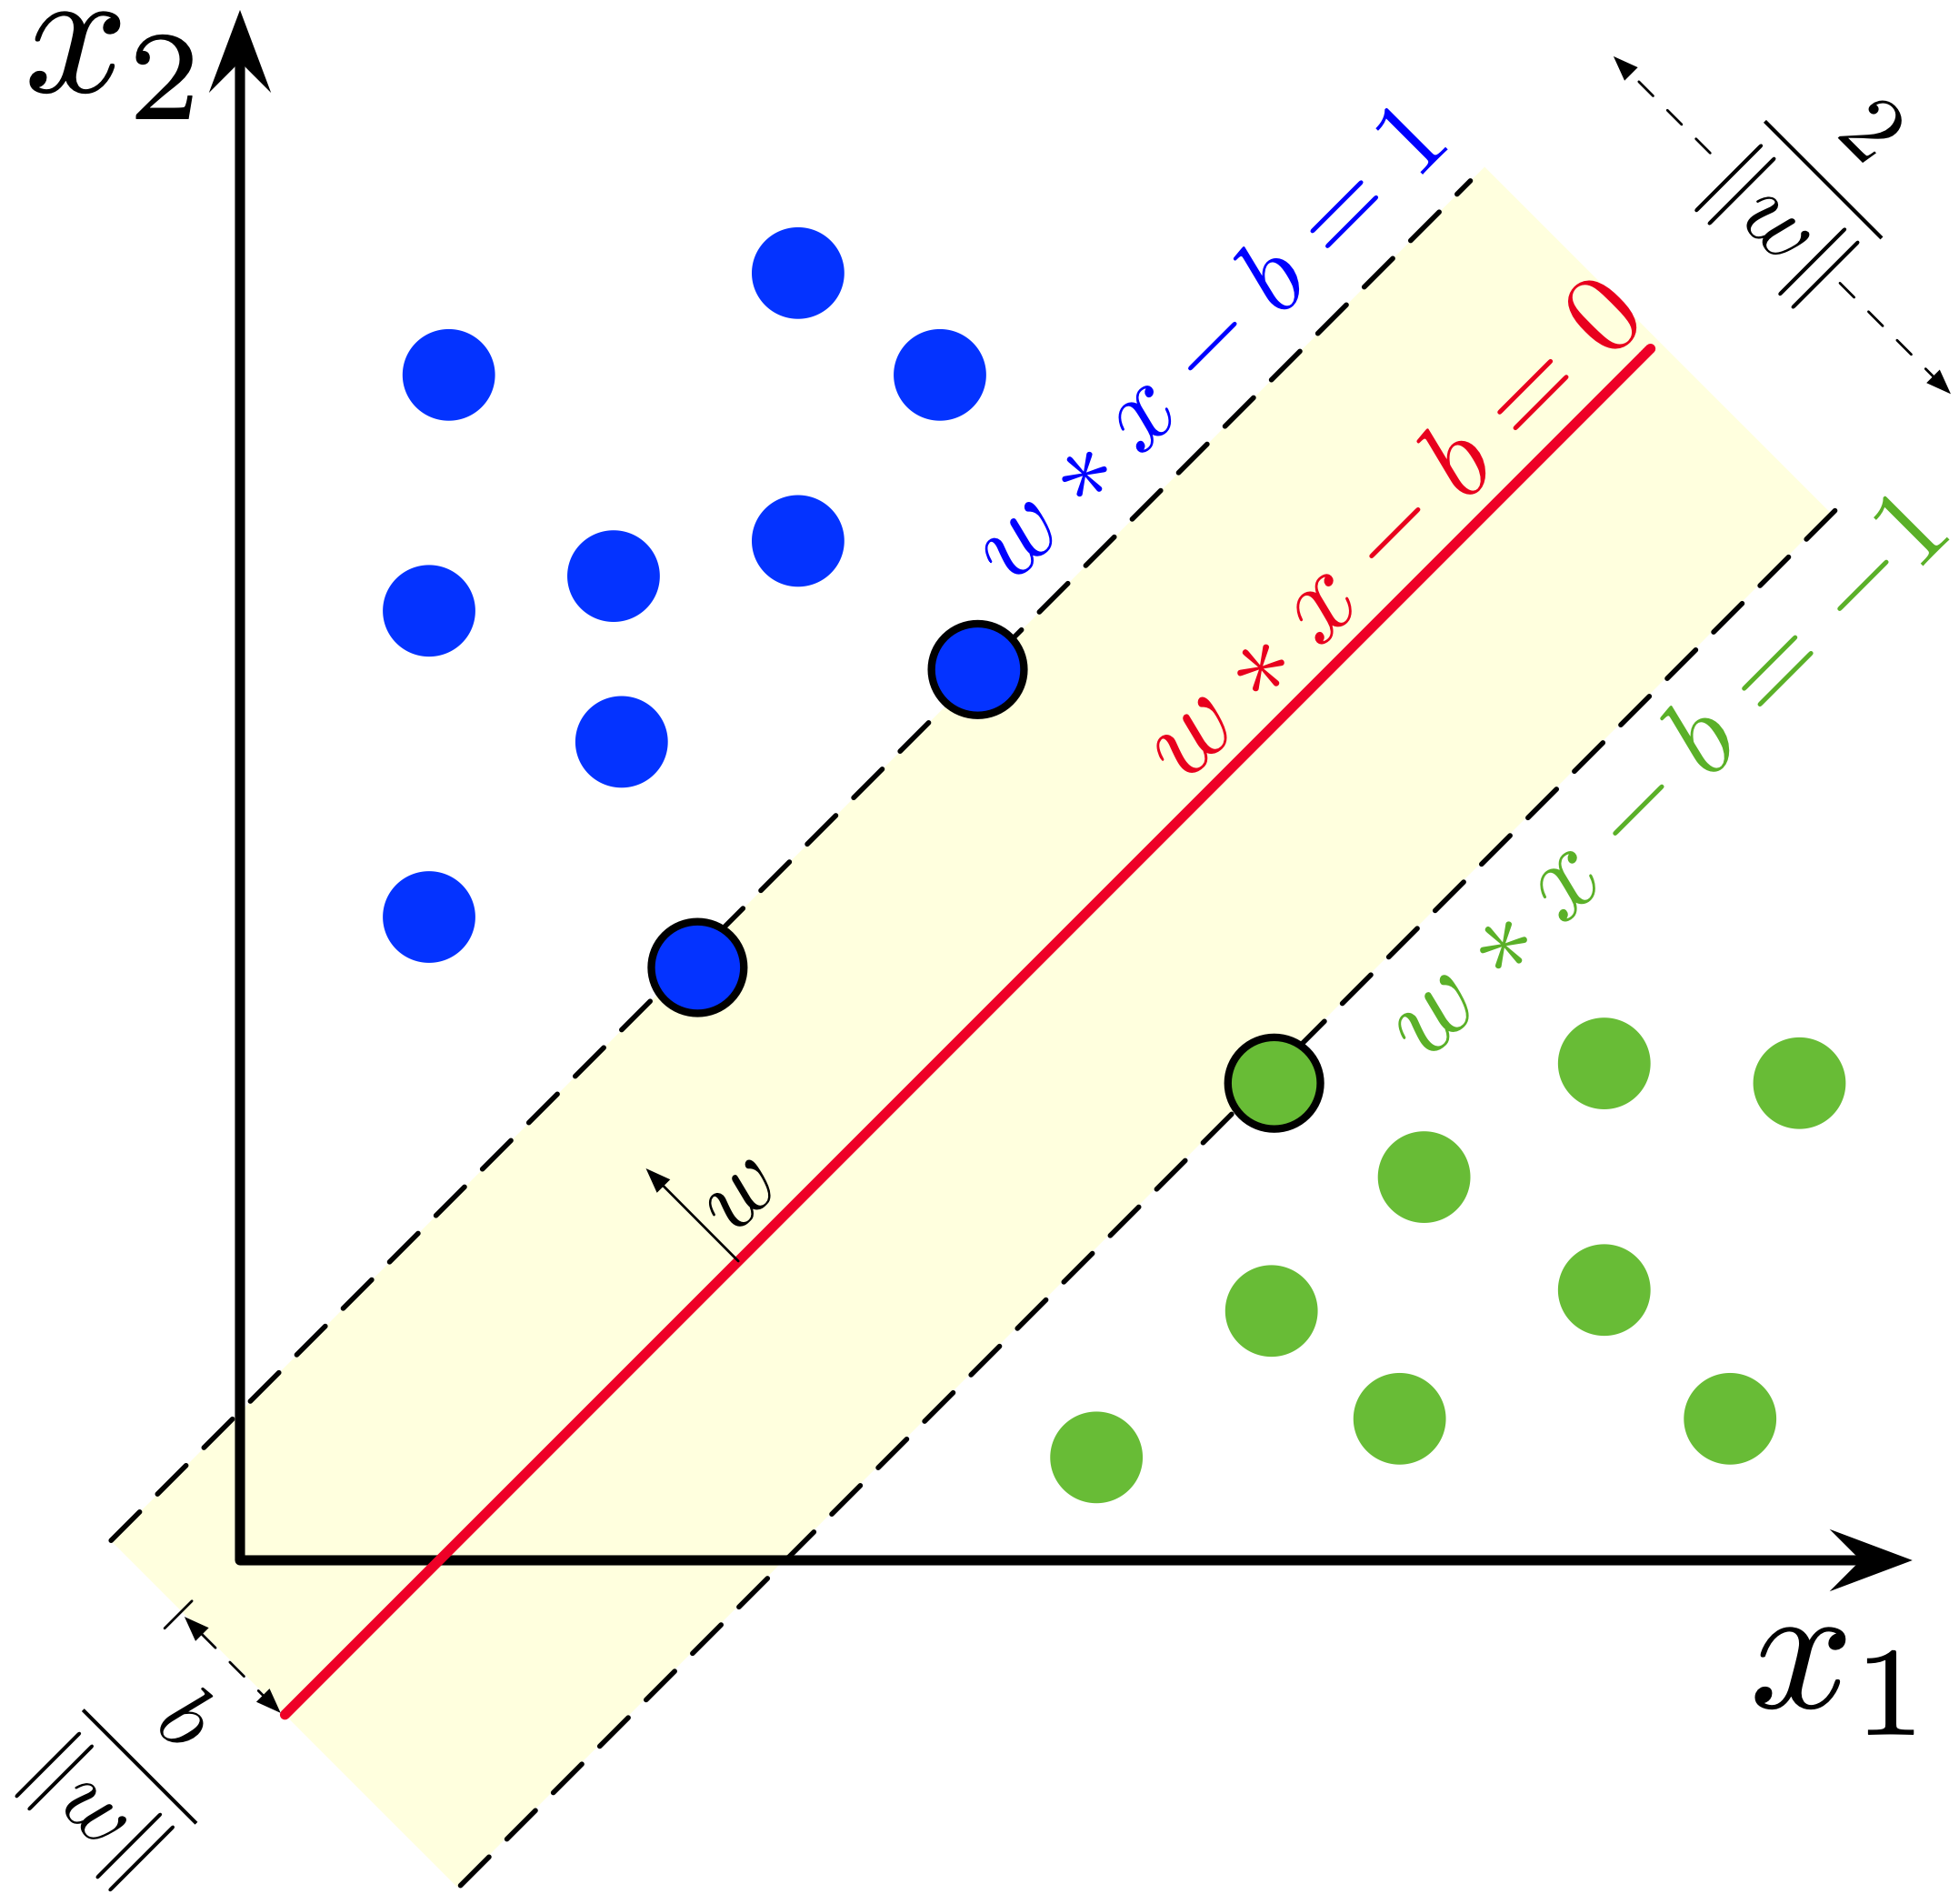
\includegraphics[width=.3\linewidth]{SVM_margin.png}
% 	\caption{}
% \end{figure}
construct the classifier
\begin{equation}
	\tilde{m}(\vb{s}) := \textup{sign} \qty(
		\sum_{i=1}^t y_i \alpha_i^* \kernel(\vbx_i,\vb{s}) + b
	)
\end{equation}

\subsubsection{Quantum machine learning}\label{sec:quantum_machine_learning}
\cite{biamonteQuantumMachineLearning2017}; neural network

\subsection{Group theory and symmetries}
group $\group$

\subsubsection{Representation theory}\label{sec:representation_theory}

\section{Symmetries in physics}
\subsection{Lagrangian formalism}\label{sec:lagrangian}
\subsubsection{Path integral and quantum computing}
\cite{xuLagrangianFormalismQuantum2021}
In optics, Fermat's principle states that the path taken by a ray between two given points is the path that can be traveled in the least (extremum) time. 
% Lagrange multiplier method
A similar argument, \emph{principle of least action}, was developed in classical mechanics:
% [\emph{Principle of least action}]
% postulate
% \begin{postulate}
% \end{postulate}
\begin{axiom}[Principle of least action]\label{thm:least_action}
    The actual path $q(t)$ taken by a classical system is the path that 
	yields an extremum of its action \(\action\).
	So, this principle is also called principle of stationary action.
	% or \emph{Hamilton's principle}.
	The action of the dynamics is the integral of Lagrangian over time
	\begin{equation}
		\action[q(t)]:=\int_{t_I}^{t_F}\dlagrangian(q(t),\dot{q}(t);t)\dd{t}
		\label{eq:action}
	\end{equation}
	where $\lagrangian(q,\dot{q})$ is the Lagrangian in terms of generalized coordinate $q$ and velocity $\dot{q}$ at certain time $t$. 
\end{axiom}
The notion $\action[\cdot]$ reminds that action is a functional that takes a function (path) $q(t)$ as input.
% see \cref{sec:path_integral} for more detail.
% (the simplest case is cartesian corrdinates, can be spherical etc)
% In classical mechanics, it is the actual path in the Euclidean space. 
By varying the action, one have the equation of motion (Eq.\ref{eq:euler_lagrange}) called \emph{Euler-Lagrange equation}.
% \begin{equation}
%     \pdv{\lagrangian}{q_a}-\dv{t}\pdv{\lagrangian}{\dot{q}_a}=0
% \end{equation}
This Lagrangian formalism was extended by Dirac \cite{diracAnalogyClassicalQuantum1945} and Feynman \cite{feynmanQuantumMechanicsPath2010} to explain quantum mechanics. 
\begin{axiom}[Path integral]\label{thm:path_integral}
    The amplitude (probability) of a quantum system evolving from $\ket{q_I}$ to $\ket{q_F}$ in a time interval can be evaluated by (functional) integrating over all possible paths with fixed initial and final position 
    \begin{equation}
		\mel{q_F}{e^{-\ii t\hhat/\hbar}}{q_I} =
        \int_{q(t_I)= q_F}^{q(t_F)=q_I} \D q \; e^{\ii \action[q]/\hbar}
    \end{equation}
	where the action defined in classical mechanics as \cref{eq:action}.
\end{axiom}
The Larangian (path integral) formalism of quantum mechanics is proved to be equivalent to the well-known \schrodinger equation \cref{eq:evolution} \cite[Chp4]{feynmanQuantumMechanicsPath2010} 
% (complete specification)
% \begin{equation}
%     \ii\hbar \dv{t} \ket{\psi(t)} = \hhat(t) \ket{\psi(t)}
% 	% \ket{\psi}=\sum_{q} \alpha_{q} \ket{q}$, $\sum_{q} \abs{\alpha_{q}}^2=1.
%     \label{eq:evolution}
% \end{equation}
which is a differential equation determining the evolution of quantum state.
In the classical limit (Planck's constant $\hbar\to 0$), \nameref{thm:path_integral} reduces to \nameref{thm:least_action}
because only the paths around the stationary point of the action contribute 
(the other paths' contributions frequently oscillate and cancel out).
% We have included a summary of the path integral formalism for various kinds of systems in \cref{sec:path_integral}.

\subsection{Symmetries with Lagrangian}